\section{Majorana fermions and topological superconductors}

Before we define Majorana fermions we will discuss characteristics of fermions.
There are three types of fermions: Dirac, Weyl, Majorana.
Both Enrico Fermi and Paul Dirac derived Fermi-Dirac statistics, independently and roughly the same time in 1926.
Fermions are particles that follow Fermi-Dirac statistics and the Pauli exclusion principle and have half-integer spin (spin 1/2, 3/2, etc.).
Dirac's equation led to the derivation of a (complex) wavefunction solution for spin-half fermions that have mass and charge, and an antiparticle, coined as the positron.
A few years later, Hermann Weyl derived from Dirac's equation a simplified solution for describing massless fermions.
Then, in 1937 Ettore Majorana hypothesized from Dirac's equation a (real) wavefunction solution that showed that these fermions were both particle and antiparticle and neutrally charged.

Examples of observed fermions include electrons, neutrinos, neutrons, and protons.
Weyl and Majorana fermions have yet to be observed.
The Standard Model does allow for neutrinos to potentially be Majorana fermions.
The MAJORANA project: neutrinoless double beta decay, is one experiment for detecing neutrino Majorana fermions and has yielded negative results thus far.
The particle physics community has not found either Weyl and Majorana fermions in any experiment yet.
There are, however, avenues for pursuing them as quasiparticles in condensed matter systems.
For example, in 2011 Weyl fermions were theorized to be in topological semimetals then quickly observed by 2015 in TaAs semimetals using angle-resolved photoemission spectroscopy (ARPES)  ~\cite{wanTopologicalSemimetalFermiarc2011, xuDiscoveryWeylFermion2015, liWeylSemimetalTaAs2016}.

To understand where Majorana fermions come from lets look at what quasiparticles exist in superconductors.
Since 2001 it has been hypothsized that Majorana fermions can be found on \textit{p}-wave superconductors in pairs of 2 and non-localized in half-quantum vortices and at the ends of wires  ~\cite{ivanovNonAbelianStatisticsHalfQuantum2001, kitaevUnpairedMajoranaFermions2001}.
In conventional superconductors there are cooper pairs that make up the supercurrent.
These Cooper pairs are made up of two electrons (or holes) with opposite spin and momenta caused by the electron-phonon interaction, are bosonic and condensate, and are in a ground state with allowed excited states.
A Bogoliubov quasiparticle is the first excited state of a Cooper pair condensate, this is when an electron and hole with opposite momenta become paired.
This usually happens when the systems chemical potential allows the electron and hole bands to cross one another in the brillouin space and the superconducting order parameter, $\Delta$, dictates the type of spin coupling.
For example, superconductors that are \textit{s}-wave pair electrons and holes with opposite spin, while \textit{p}-wave pairs electrons and holes that are spin-polarized or spinless.
In a \textit{p}-wave superconductor if the Bogoliubov quasiparticle is a zero-energy excitation it can be written as a Majorana fermion and because of the particle-hole symmetry in the system they come in pairs.
\Blue{Should I mention anything about singlets and triplets and mention a generalized 2$\times$2 d vector notation for order parameter?}

\Blue{We have yet to physically realize a $p$-wave superconductor experimentally, however, we can use heterostructures in proximity to an $s$-wave superconductor to achieve an effective $p$-wave superconduting interface, which is explained and referenced in later chapters.}
\Blue{Majorana fermions are dictated by non-Abelian exchange statistics, which allows for building a universal quantum computer, hence why they are highly sought after.}
\Blue{Another boon of using a non-trivial topological superconductor is the ability to protect Majorana fermions from local perturbations.}

\subsection{Kitaev chain}
Ivanov first showed how to derive Majorana fermions in a 2D \textit{p}-wave superconductor.
However, we find it easier to understand Kitaev's approach first.
Let us go ahead and show how Kitaev derived Majorana zero modes (MZMs), Majorana(MFs), on a 1D spinless $p$-wave superconductor.
Start with a 1D spinless $p$-wave superconductor tight-binding Hamiltonian

\begin{equation}
  \ham = \sum_j^{N-1} (-t \cc_j c_{j+1} + \Delta c_j c_{j+1} + h.c.) - \sum_j^{N} \mu \cc_j c_j,
\end{equation}
where $t$ is hopping amplitude, superconducting order parameter $\Delta = |\Delta|$ for simplicity, $\mu$ is chemical potential, and $\cc (c)$ is the creation (annihilation) operator for a complex fermion.
We use a basis tranformation to convert to the Majorana fermion basis, where
$\cc_j = \tfrac{1}{2} (a_j - i b_j)$, $\left\{ a^{\dagger}_j, a_{j'} \right\} = \left\{ a_j, a_{j'} \right\} = 2\delta_{j,j'}$
since they are Majorana fermions, and $\left\{a_j,b_j'\right\} = 0$.
After some algebra we arrive at

\begin{equation}
  \ham = \dfrac{i}{2} \sum_j \left( -\mu a_j b_j + (t+\Delta) b_j a_{j+1} + (-t+\Delta) a_j b_{j+1} \right).
\end{equation}
In the trivial topology phase, there are no Majorana fermions, $\mu \neq 0$ and $t=\Delta=0$,

\begin{equation}
  \ham = -\mu\dfrac{1}{2} \sum_j a_j b_j.
\end{equation}
For non-trivial topology phase, there are Majorana fermions present, $\mu = 0$, and $t = \Delta > 0$,

\begin{equation}
  \ham = it \sum_j b_j a_{j+1}.
\end{equation}
Notice the terms $a_0$ and $b_N$ are missing in the non-trivial topology Hamiltonian, we can say there is a non-localized zero energy mode present in the system defined by $f = \tfrac{1}{2}(a_0 + i b_N)$, hence the name Majorana zero modes.
Figure ~\ref{fig:kitaev-chain} shows the wire in both topological phases.
One quick note on terminology, sometimes non-trivial topology is referred to as the topological phase, for the purposes of this dissertation we will use the former option.
Now, slightly outside the Kitaev limit for non-trivial topology, we can limit $|\mu| < 2t$ and $t = |\Delta| >0$ and still achieve non-trivial topology with Majorana zero modes at the interface of trivial and non-trivial topology.

\begin{figure}
  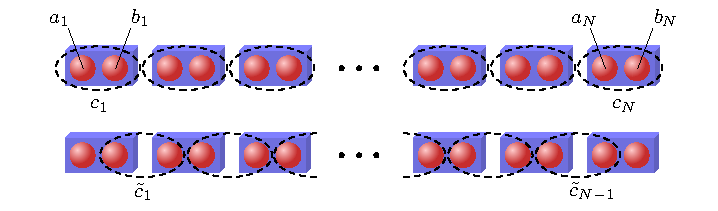
\includegraphics[width=\textwidth]{./figures/kitaev-chain.pdf}
  \caption{The top chain represents the system in a trivial topology where each complex fermion $c_j = \tfrac{1}{2}(a_j + i b_j)$ is a linear combination of intraconnected MFs. The bottom chain represents the system in a non-trivial topology where each complex fermion $\tilde{c}_j = \tfrac{1}{2}(a_j + i b_{j+1})$ is a linear combination of interconnected MFs, leaving the non-localized complex fermion $f = \tfrac{1}{2}(a_0 + i b_N)$, and thus leaving one MF located at each end of the chain.}
  \label{fig:kitaev-chain}
\end{figure}

To understand why this is still true we can determine the topological invariant for the system, also known as the Majorana number, a type of Winding number for 1D superconducting systems.
While calculating the Majorana number is straight forward enough, its proof on the other hand is not, this can be found in the appendix REFERENCE appendix here.
We write the Hamiltonian in the Majorana basis, $A = -iU \ham U^{\dagger}$, then take the sign of the Pfaffian,

\begin{equation}
  \mathcal{M} = \text{sgn} [\text{Pf} (A)].
\end{equation}
This calculation can be reduced down if we can write the Hamiltonian in momentum space.
Employing the following symmetry $\epsilon(-k) = -\epsilon(k)$ we find there are $n$ positive and $n$ negative eigenvalues in the system for any given $k$ value.

\begin{equation}
  \mathcal{M} =
  \begin{cases}
    \text{sgn} [\text{Pf} (A_{k=0}) \text{Pf} (A_{k=\pi})], &\text{if L is even}, \\
    \text{sgn} [\text{Pf} (A_{k=0})], &\text{if L is odd},
  \end{cases}
\end{equation}
where L is the number of lattice sites from our lattice Hamiltonian.
We find that under the Kitaev limit, if $|\mu|< 2t$, then $\mathcal{M} = -1$, and if $|\mu| > 2t$, then $\mathcal{M} = 1$.
When a section of the material is in a non-trivial topology and either the other material is trivial or vacuum, which is also trivial, Majorana zero modes will be localized at interfaces of differing topological number, this is also known as bulk-edge correspondence and will be used later in our topological quantum logic gate.
As a last note, when $|\mu| = 2t$ this is a critical point and where the gap opens and closes, it is not an ideal region of parameter space for the band gap is too small ~\cite{kitaevUnpairedMajoranaFermions2001}.
*Originally, Kitaev's proposal was to design topological quantum storage.

\subsection{Half-quantum vortices in \textit{p}-wave superconductors}
We now transition back to Ivanov's derivation of MFs and begin to introduce \textit{braiding} for topological quantum computing as a key reason for hosting and manipulating MFs.
It was proposed by Read and Green that the Pfaffian quantum Hall state derived by Moore and Read belongs to the same topological class as the BCS pairing state.
Ivanov then verified this was the case for a BCS pairing state.
Since the Pfaffian state was shown to exhibit non-Abelian statistics for half-quantum vortices the same is true for \textit{p}-wave superconductors.
To answer why this is the case we need to understand how the superconducting order parameter acts for different pairing potentials composing of singlet or triplet states.

The superconducting order parameter, called order parameter or pairing potential for short, tells us the correlation between two fermionic operators in a superconductor and thus requires the state to be antisymmetric.
These states are made up of a spatial and spin component.
When the two electrons in a cooper pair are a spin-singlet the spin component is antisymmetric and requires the spatial component be symmetric; this occurs in \textit{s}- and \textit{d}-wave superconductors.
If instead the electrons in a cooper pair are a spin-triplet the spin component is symmetric and requires the spatial component by antisymmetric; this occurs in \textit{p}- and \textit{f}-wave superconductors.
In terms of Pauli matrices we can in general encode the order parameter with

\begin{equation}
  \Delta (\vec{k}) = \left(\Delta_0 (\vec{k}) + \vec{d}(\vec{k}) \cdot \bm{\sigma}\right) i \sigma_y,
\end{equation}
with the following antisymmetric definition $\Delta(\vec{k}) = \Delta^T(-\vec{k})$, we see $\Delta_0 (\vec{k})$ encodes spin-singlet components and $\vec{d}(\vec{k})$ encodes spin-triplet components, and at the end $\sigma_y$ is there to keep the matrix antisymmetric.
The direction vector $\vec{d}$ needs to be a three dimsensional vector to ensure we account for the three spin configurations
$|\uparrow\uparrow\rangle$, $|\uparrow\downarrow\rangle + |\downarrow\uparrow\rangle$, and $|\downarrow\downarrow\rangle$.
To account for even-parity in the symmetric spatial component the momentum is of even powers proportional with the even spherical harmonics, while odd-parity in the antisymmetric component the momentum is of odd powers proportional to the odd spherical harmonics.
For example, in \textit{s}-wave superconductors, $l=0$ and $Y_{0,0} = \text{const.}$ and has no momentum dependence and
$\Delta_s (\vec{k}) = i\Delta_0 \sigma_y$.
In the case of \textit{p}-wave superconductors, $l=1$ and $Y_{1,\pm1} \propto k_x \pm i k_y$ leading to linear dependence in momentum such that the order parameter becomes
$\Delta_p(\vec{k}) = i\Delta (\vec{d} \cdot \bm{\sigma}) (k_x+ik_y) \sigma_y$.

\begin{figure}
  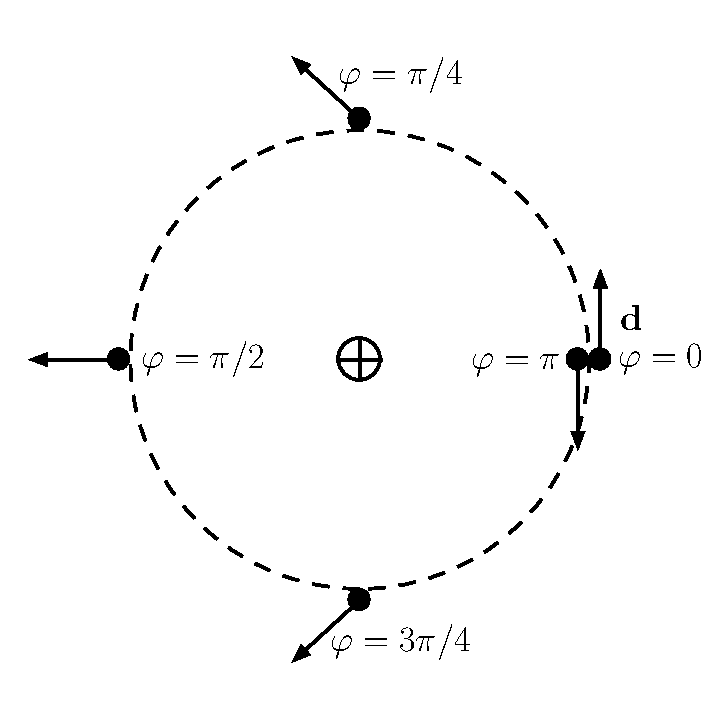
\includegraphics[width=0.4\textwidth]{./figures/half-quantum-vortex.pdf}
  \caption{The order phase $\varphi$ and angle $\alpha$ of $\vec{d}$ rotate by $\pi$: ($\varphi , \vec{d}$) \rightarrow ($\varphi+\pi, -\vec{d}$). The order parameter $\theta$ maps to itself, ($0, 2\pi$), under simultaneous change of both $\vec{d}$ and $\varphi$: $\theta = \varphi + \alpha$.}
  \label{fig:half-quantum-vortex}
\end{figure}

In Ivanov's case he picked a slightly different basis for the triplet-pairing order parameter,

\begin{equation}
  %\Delta (\vec{k}) = \Delta e^{i\phi} \left[ d_x \left(|\uparrow\uparrow\rangle + |\downarrow\downarrow\rangle \right) +i d_y \left(|\uparrow\uparrow\rangle - |\downarrow\downarrow\rangle \right) + d_z \left(|\uparrow\downarrow\rangle + |\downarrow\uparrow\rangle \right) \right] (k_x + i k_y),
  \Delta (\vec{k}) = \Delta e^{i\varphi} \left[ d_x \sigma_0 + i d_y \sigma_z + d_z \sigma_x \right] (k_x + i k_y)
\end{equation}
it still follows the antisymmetric definition
$\Delta(\vec{k}) = -\Delta^T (-\vec{k})$.
For a half-quantum vortex to exist, we must allow $\vec{d}$ to rotate in 3D or on a plane.
Additionally, the order parameter maps to itself, which requires the change of sign of $\vec{d}$ and shift in the phase $\varphi$ by $\pi$ simultaneously.
This mapping is
$(\varphi, \vec{d}) \mapsto (\varphi+\pi,-\vec{d})$
and can be seen in Figure ~\ref{fig:half-quantum-vortex}.

We now reduce to a 2D superconductor, this forces $\vec{d}$ to point and rotate in the x-y plane and removes the coupling of spin-up and -down fermions from the order parameter.
The order parameter can then be written in polar coordinates

\begin{align}
  \Delta (\vec{k},r,\theta) &= \Delta(r) e^{i\varphi}
  \begin{bmatrix}
    e^{i\alpha} & 0 \\
    0 & e^{-i\alpha}
  \end{bmatrix}
  (k_x + i k_y) \nonumber \\
  &= \Delta(r)
  \begin{bmatrix}
    e^{i\theta} & 0 \\
    0 & 1
  \end{bmatrix}
  (k_x + i k_y),
\end{align}
where $\alpha$ is the angle of $\vec{d}$, remembering its simultaneous change w.r.t. $\varphi$.
We see that the spin-up fermions have a vortex while the spin-down do not have a vortex (and thus no low energy states).
The Hamiltonian for spin-up or spinful fermions can now be described by

\begin{equation}
  \ham = \int d^2 \vec{r} \left[ -\Psi^{\dagger} \left( \dfrac{\nabla^2}{2m} + \epsilon_F \right) \Psi + \Psi^{\dagger} \left[ e^{i\theta} \Delta(r) * \left( \partial_x +i\partial_y \right) \right] \Psi^{\dagger} + h.c. \right],
\end{equation}
where $*$ is the symmetrized product
[$A*B = (AB + BA) / 2$].
One can diagonlize the Hamiltonian using the quasiparticle operator
$\gamma^{\dagger} = u\Psi^{\dagger} + v\Psi$.
The creation annihilation of the same fermion is related by the parameters $u$ and $v$, causing the energy eigenstates to be symmetric about zero-energy forcing
$\gamma^{\dagger}(E) = \gamma (E)$.
It then leads to the zero-energy eigenstate being self-conjugate, a Majorana fermion,
$\gamma^{\dagger}(E=0) = \gamma (E=0)$.
The spinful nature eliminates the spin degree of freedom and shows the creation and annihilation operators are coupled due to superconductivity, making the Majorana fermion possible through self-conjugacy.

\subsection{Braiding}
Let us now talk about gauge symmetry.
Under \textit{U}(1) gauge transformation, if the superconducting gap is shifted by $\phi$, it is the same as rotating the creation annihilation operator by half the shift.
Thus, $\Psi_{\alpha} \mapsto e^{i\phi/2} \Psi_{\alpha}$, which leads to the Majorana fermion operator weights transforming as $(u,v) \mapsto (ue^{i\phi/2}, v^{-i\phi/2})$.
We can see with a change of superconducting order parameter by $2\pi$ the Majorana fermion changes sign, $\gamma \mapsto -\gamma$.

\begin{figure}
  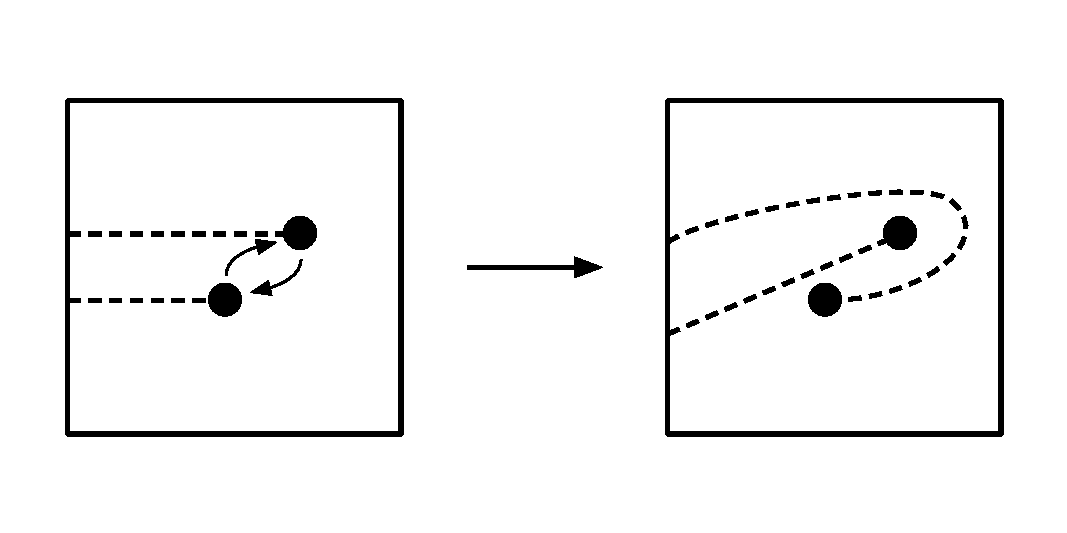
\includegraphics[width=0.5\textwidth]{./figures/pwave-braid.pdf}
  \caption{Two vortices in an elementary braid exchange.}
  \label{fig:pwave-braid}
\end{figure}


This change of sign is important in braiding transformations since it allows for non-Abelian statistics.
We can circumvent a global phase by introducing branch cuts for the vortices to cross, causing a $2\pi$ phase change in the Majorana fermion.
Vortices can be exchanged as described in Figure ~\ref{fig:pwave-braid}, with a "bird's eye" view.
We can define the braiding operators as the following

\begin{equation}
  T_i :
  \begin{cases}
    \gamma_i \mapsto \gamma_{i+1} \\
    \gamma_{i+1} \mapsto -\gamma_i \\
    \gamma_j \mapsto \gamma_j \quad\quad \text{for $j\neq i$ and $j\neq i+1$}.
  \end{cases}
\end{equation}
This leads us to the following braiding relations

\begin{figure}
  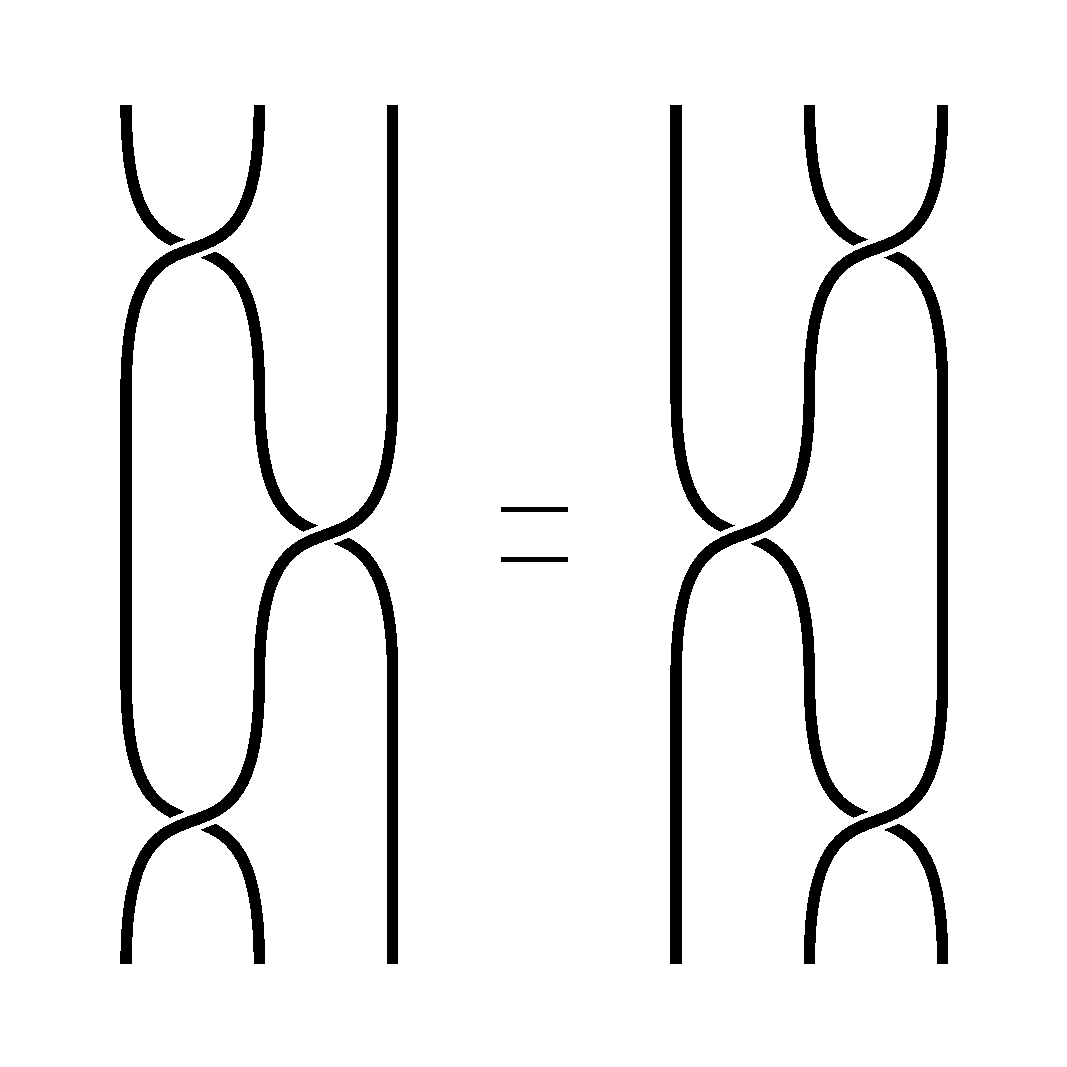
\includegraphics[width=0.33\textwidth]{./figures/braid.pdf}
  \caption{Braid group relation for $T_i T_{i+1} T_i = T_{i+1} T_i T_{i+1}$.}
  \label{fig:braid}
\end{figure}
\begin{equation}
  \begin{align*}
    T_i T_j = T_j T_i, \quad |i-j| > 1, \\
    T_i T_j T_i = T_j T_i T_j, \quad |i-j| = 1.
  \end{align*}
\end{equation}
Figure ~\ref{fig:braid} demonstrates three neighboring vortices and their braiding statistics having two means of achieving the same braiding exchange.
One can write the braiding operators in terms of fermionic operators with the following

\begin{equation}
  \tau(T_i) = \exp\left(\dfrac{\pi}{4} \gamma_{i+1} \gamma_i\right) = \dfrac{1}{\sqrt{2}} \left(1+ \gamma_{i+1} \gamma_i\right).
\end{equation}
This can be further carried out for a number of Majorana fermions and builds a set of braiding operators for that system ~\cite{ivanovNonAbelianStatisticsHalfQuantum2001}.

\subsection{T-junction qubit}
The simplest qubit theorized for braiding Majorana fermions is on 1D wires connected in a T-junction, which can be extrapolated to a ladder junction for $2n$ Majorana fermions.
In the T-junction we define the quasi-1D Hamiltonian

\begin{equation}
  \ham = -\mu \sum_j \cc_j c_j - \sum_j \left(t\cc_j c_{j+1} + |\Delta|e^{i\phi} c_j c_{j+1} + h.c. \right),
\end{equation}
where
$c_j = e^{-i\phi/2} (\gamma_{j+1,1} + i \gamma_{j,2})/2$.
We additionally have to define the pairing as
$|\Delta|e^{i\phi} c_j c_{j+1}$
such that the site indices have the following definitions
\begin{itemize}
  \item Increase moving $\rightarrow / \uparrow$ in the horizontal/vertical wires: $\phi = 0$,
  \item Decrease moving $\leftarrow / \downarrow$ in the horizontal/vertical wires: $\phi = \pi$.
\end{itemize}
The braiding of two Majorana fermions in a T-junction is achieved by adiabatically tuning the voltage gate, or chemical potential, of the wires which can be seen in Figure ~\ref{fig:t-junction-braid}
Then we can extroplate to a ladder junction as shown in Figure ~\ref{fig:ladder-junction} ~\cite{aliceaNonAbelianStatisticsTopological2011}.
While this approach is simple in theory and being seriously pursued, it is difficult to build, manipulate, and read experimentally.
Another difficulty for these wires is due to not having any truly \textit{p}-wave superconductors, currently they need to be built from heterostructures to make an effective \textit{p}-wave superconductor.

\begin{figure}
  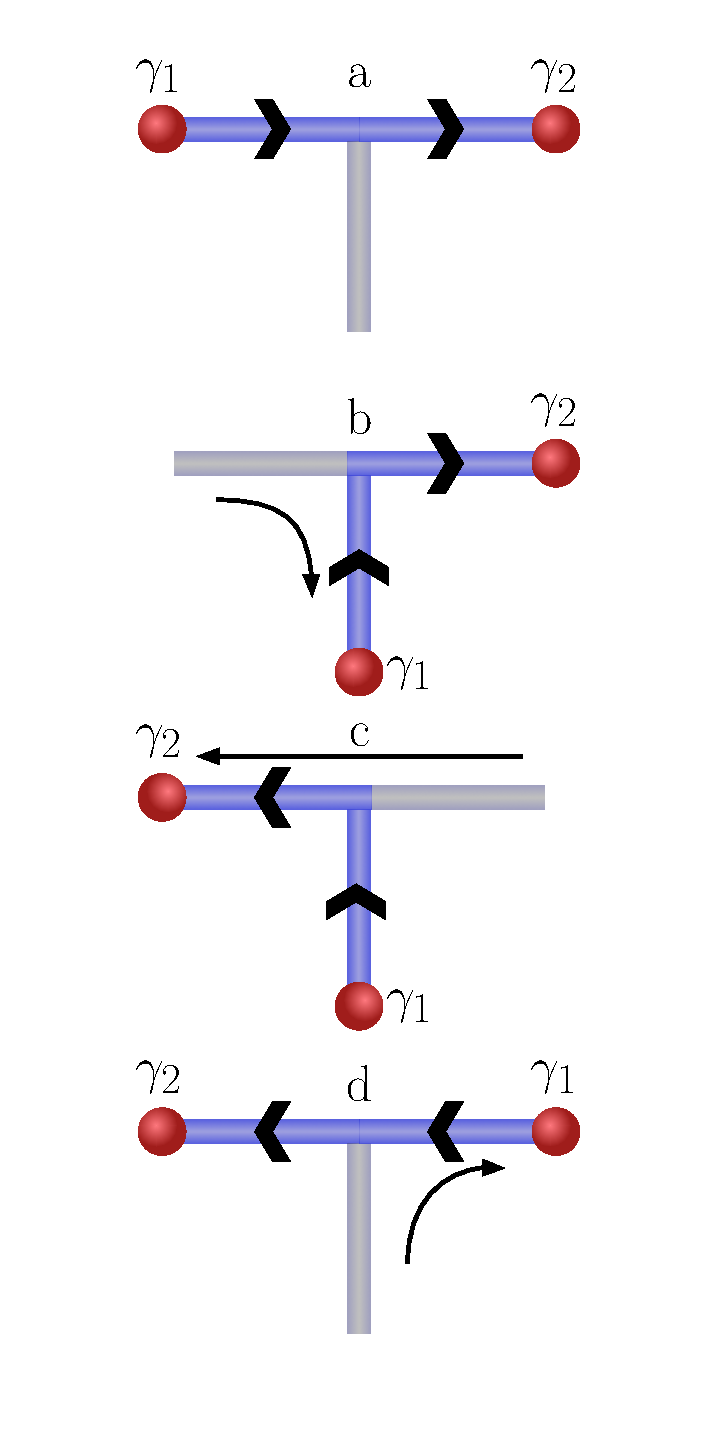
\includegraphics[width=0.3\textwidth]{./figures/t-junction-braid.pdf}
  \caption{Braiding two Majorana fermions on a T-junction.}
  \label{fig:t-junction-braid}
\end{figure}

\begin{figure}
  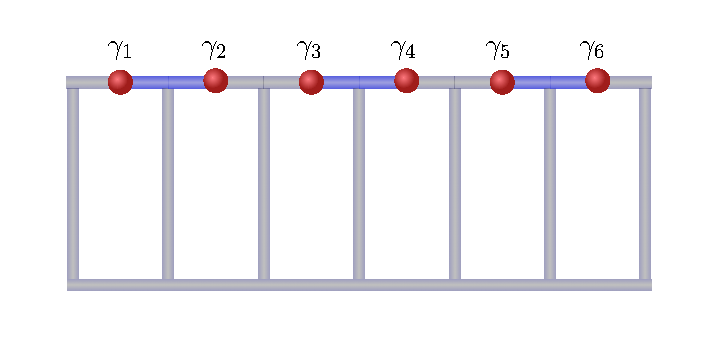
\includegraphics[width=0.5\textwidth]{./figures/ladder-junction.pdf}
  \caption{Ladder junction schematic for hosting and braiding multiple Majorana fermions.}
  \label{fig:ladder-junction}
\end{figure}

\subsection{Effective \textit{p}-wave superconductors}
There are several ways to build an effective \textit{p}-wave superconductor.
We go over one example given by Sau et.\ al. ~\cite{sauGenericNewPlatform2010}.
A zinc-blende semiconductor quantum well grown along the (100) direction is considered. We start with the relevant noninteracting Hamiltonian

\begin{equation}
  \ham_0 = \sum_{\vec{k}}  \cc_{\vec{k}} \left[\frac{k^2}{2m} - \mu + \alpha ( \sigma^x k_y - \sigma^y k_x) \right] c_{\vec{k}}
\end{equation}
where $m$ is the effective mass, $\mu$ is the chemical potential, $\alpha$ is the Rashba spin-orbit(REFERENCED in Alicea's paper as ref 23) coupling strength, and $\sigma^i$ are the Pauli matrices that act on the spin degrees of freedom in $c_{\vec{k}}$. We have set $\hbar=1$ throughout.

We next introduce a ferromagnetic insulator and a magnetic field. The ferromagnetic insulator has magnetization pointing perpendicular to the 2D semiconductor.

\begin{equation}
  \ham_Z = V_z \sum_{\vec{k}} \cc_{\vec{k}} \sigma^z c_{\vec{k}}
\end{equation}
but neglible orbital coupling. If we look at the combined Hamiltonian it becomes obvious there is a constant energy plus the energy eigenvalues of the Pauli matrices terms. We can easily solve the eigenvalue problem of

\begin{equation}
  \begin{bmatrix}
    V_z & \alpha (k_y + i k_x) \\
    \alpha (k_y -i k_x) & -V_z
  \end{bmatrix}
\end{equation}
giving $\epsilon_{\pm}'(\vec{k}) = \pm \sqrt{V_z^2+\alpha^2 k^2}$ with eigenvectors

\begin{align}
  u_+(\vec{k})  =
  \left( \begin{array}{l}
      A_\uparrow(\vec{k}) \\
      -A_\downarrow(\vec{k}) \dfrac{k_y - i k_x}{k}
  \end{array} \right)
  \\ \\
  u_-(\vec{k})  =
  \left( \begin{array}{l}
      B_\uparrow(\vec{k}) \dfrac{k_y + i k_x}{k}  \\
      B_\downarrow(\vec{k})
  \end{array} \right)
\end{align}
One can find $A_{\sigma}=A_{\sigma}^*$ and $B_{\sigma}=B_{\sigma}^*$ and the coefficients are

\begin{align}
  A_{\uparrow}(\vec{k}) &= \dfrac{-\alpha k}{\sqrt{2\epsilon_+'(\vec{k})}} \sqrt{\dfrac{1}{\epsilon_+'(\vec{k})-V_z}} \\
A_{\downarrow}(\vec{k}) &= \sqrt{\dfrac{\epsilon_+'(\vec{k})-V_z}{2\epsilon_+'(\vec{k})}} \\
B_{\uparrow}(\vec{k}) &= \sqrt{\dfrac{\epsilon_-'(\vec{k})+V_z}{2\epsilon_-'(\vec{k})}} \\
B_{\downarrow}(\vec{k}) &= \dfrac{\alpha k}{\sqrt{2\epsilon_-'(\vec{k})}} \sqrt{\dfrac{1}{\epsilon_-'(\vec{k})+V_z}}
\end{align}
The expressions for $A_{\uparrow,\downarrow}$ and $B_{\uparrow,\downarrow}$ can be written in convenient terms as

\begin{align}
  f_p(\vec{k}) &= A_{\uparrow}(\vec{k})A_{\downarrow}(-\vec{k}) = B_{\uparrow}(-\vec{k})B_{\downarrow}(\vec{k}) \\
  &= \dfrac{-\alpha k}{2\epsilon_+'(\vec{k})}
\end{align}

When putting the semiconductor in contact with an $s$-wave superconductor a pairing term is generated by the proximity effect. The full Hamiltonian becomes $\mathcal{H} = \mathcal{H}_0 + \mathcal{H}_Z + \mathcal{H}_{SC}$ with

\begin{align}
  \mathcal{H}_{SC} = \sum_{\vec{k}} \Delta c_{\uparrow,\vec{k}}^\dagger c_{\downarrow,-\vec{k}}^\dagger + H.c.
\end{align}

We now want to write the pairing potential in terms of $c_{\pm}$ using a basis transformation.

\begin{align}
  c_{\uparrow,\vec{k}} &= \bra{\uparrow}\ket{u_+(\vec{k})} c_{\vec{k},+} + \bra{\uparrow}\ket{u_-(\vec{k})} c_{\vec{k},-} \\
  &= A_{\uparrow}(\vec{k}) c_{\vec{k},+} + B_{\uparrow}(\vec{k})\dfrac{k_y+i k_x}{k} c_{\vec{k},-} \\
  c_{\downarrow,-\vec{k}} &= \bra{\downarrow}\ket{u_+(-\vec{k})} c_{-\vec{k},+} + \bra{\downarrow}\ket{u_-(-\vec{k})} c_{-\vec{k},-} \\
  &= A_{\downarrow}(-\vec{k})\dfrac{k_y-i k_x}{k} c_{-\vec{k},+} + B_{\downarrow}(-\vec{k}) c_{-\vec{k},-}
\end{align}
with the adjoints being

\begin{align}
  \cc_{\uparrow,\vec{k}} &= A_{\uparrow}(\vec{k}) \cc_{\vec{k},+} + B_{\uparrow}(\vec{k})\dfrac{k_y-i k_x}{k} \cc_{\vec{k},-} \\
  \cc_{\downarrow,-\vec{k}} &= A_{\downarrow}(-\vec{k})\dfrac{k_y+i k_x}{k} \cc_{-\vec{k},+} + B_{\downarrow}(-\vec{k}) \cc_{-\vec{k},-}
\end{align}
Continue reducing the pairing potential which becomes

\begin{equation}
  \begin{split}
    \Delta \cc_{\uparrow,\vec{k}} \cc_{\downarrow,-\vec{k}} = \Delta [ & A_{\uparrow}(\vec{k})A_{\downarrow}(-\vec{k})\dfrac{k_y+i k_y}{k} \cc_{\vec{k},+} \cc_{-\vec{k},+} + B_{\uparrow}(\vec{k})B_{\downarrow}(-\vec{k})\dfrac{k_y-i k_y}{k} \cc_{\vec{k},-} \cc_{-\vec{k},-} \\
  + & \left(A_{\uparrow}(\vec{k})B_{\downarrow}(-\vec{k})+B_{\uparrow}(\vec{k})A_{\downarrow}(-\vec{k}) \right) \cc_{\vec{k},+} \cc_{-\vec{k},-} ]
  \end{split}
\end{equation}
We will use a more convenient notation by making the following substitutions

\begin{align}
  \Delta_{++}(\vec{k}) &= \Delta f_p(\vec{k}) \dfrac{k_y +i k_x}{k} \\
  \Delta_{--}(\vec{k}) &= \Delta f_p(-\vec{k}) \dfrac{k_y -i k_y}{k} \\
  \Delta_{+-}(\vec{k}) &= \Delta f_s(\vec{k})
\end{align}
Where

\begin{align}
  f_s(\vec{k}) = \left(A_{\uparrow}(\vec{k})B_{\downarrow}(-\vec{k})+B_{\uparrow}(\vec{k})A_{\downarrow}(-\vec{k})\right)
\end{align}
The pairing potential Hamiltonian then becomes

\begin{align}
  \mathcal{H}_{SC} = \sum_{\vec{k}} \Delta_{++}c_{\vec{k},+}^{\dagger}c_{-\vec{k},+}^{\dagger} + \Delta_{--}c_{\vec{k},-}^{\dagger}c_{-\vec{k},-}^{\dagger} +\Delta_{+-}c_{\vec{k},+}^{\dagger}c_{-\vec{k},-}^{\dagger} + h.c.
\end{align}
Writing the full Hamiltonian in matrix form we will use the following Nambu spinor

\begin{align}
  \Psi = (c_{\vec{k},+},\ c_{\vec{k},-},\ c_{-\vec{k},+}^{\dagger},\ c_{-\vec{k},-}^{\dagger} )^T
\end{align}

Then we write the Hamiltonian as, where we have used the conventional BdG approach of applying the anticommutation relation and reindexing the momentum vetor of the second term to give

\begin{align}
  \mathcal{H} = \dfrac{1}{2}\sum_{\vec{k}} \Psi^{\dagger}H_{BdG}\Psi
\end{align}
with

\begin{equation}
  H_{BdG} =
  \begin{bmatrix}
    \epsilon_+(\vec{k}) & 0 & 2\Delta_{++}(\vec{k}) & \Delta_{+-}(\vec{k}) \\
    0 & \epsilon_-(\vec{k}) & -\Delta_{+-}(-\vec{k}) & 2\Delta_{--}(\vec{k}) \\
    2\Delta_{++}^*(\vec{k}) & -\Delta_{+-}^*(-\vec{k}) & -\epsilon_+(-\vec{k}) & 0 \\
    \Delta_{+-}^*(\vec{k}) & 2\Delta_{--}^*(\vec{k}) & 0 & -\epsilon_-(-\vec{k}) \\
  \end{bmatrix}
\end{equation}
where

\begin{equation}
  \epsilon_{\pm}(\vec{k}) = \dfrac{k^2}{2m} - \mu + \epsilon_{\pm}'(\vec{k})
\end{equation}
We can rearrange our matrix into a more block diagonal form with off terms to give

\begin{equation}
  H_{BdG} =
  \begin{bmatrix}
    \epsilon_+(\vec{k}) & 2\Delta_{++} & 0 & \Delta_{+-}(\vec{k}) \\
    2\Delta_{++}^* & -\epsilon_+(-\vec{k}) & -\Delta_{+-}^*(-\vec{k}) & 0 \\
    0 & -\Delta_{+-}(-\vec{k}) & \epsilon_-(\vec{k}) & 2\Delta_{--} \\
    \Delta_{+-}^*(\vec{k}) & 0 & 2\Delta_{--}^* & -\epsilon_-(-\vec{k}) \\
  \end{bmatrix}
\end{equation}
Upon studying $V_z \gg \alpha$ we see that near the fermi surface the interband pairing has little affect on the band gap. Scaling it's effect from $0 \to 1$ we see the intraband gap appears at a slightly smaller momentum as the interband pairing is turned off. We thus use the approximation $\Delta_{+-}(k_f) \approx 0$. We also set $\mu$ such that is only crosses the lower bands, thus allowing $c_+^{\dagger} \to 0$.

\begin{equation}
  H_{BdG} =
  \begin{bmatrix}
    \epsilon_-(\vec{k}) & 2\Delta_{--}(\vec{k}) \\
    2\Delta_{--}^*(\vec{k}) & -\epsilon_-(-\vec{k}) \\
  \end{bmatrix}
\end{equation}
Solving for the dispersion relation of the system we arrive at

\begin{align}
  E_{\pm}(\vec{k}) = \pm \sqrt{(\epsilon_-(\vec{k}))^2+4\abs{\Delta_{--}(\vec{k})}^2},
\end{align}
an effective \textit{p}-wave superconductor with opening and closing band gaps.

